\chapter{Configuring Digifiz Replica Next} \label{ch:Features}

\section{Panel Handling and Clock}

Replica Next instrument panels are supplied with a UV-printed polycarbonate faceplate that must be protected from scratches and sharp objects.
In the event of damage, contact the manufacturer for replacement parts; cosmetic damage is not covered by warranty.
The real-time clock is configured via the Wi-Fi control panel and resets when permanent power is removed.

\section{Accessing the Wi-Fi Control Panel}

Replica Next exposes a built-in Wi-Fi access point.
Disable mobile data on the smartphone or laptop and connect to the network named \texttt{Digifiz\_AP} (password \texttt{87654321}); some revisions use the SSID \texttt{PHOL-LABS2} with the same password.
The default IP address is \texttt{192.168.4.1}; if the panel is configured to join another network, scan the subnet for an address ending in \texttt{.32}.

Configuration, data logging, and firmware updates are provided through the embedded web application.
\Cref{fig:next-control-tabs} shows the landing page with the three primary tabs: \emph{WiFi}, \emph{Control}, and \emph{About}.

\begin{figure}[htbp]
    \centering
    \begin{subfigure}{0.48\textwidth}
        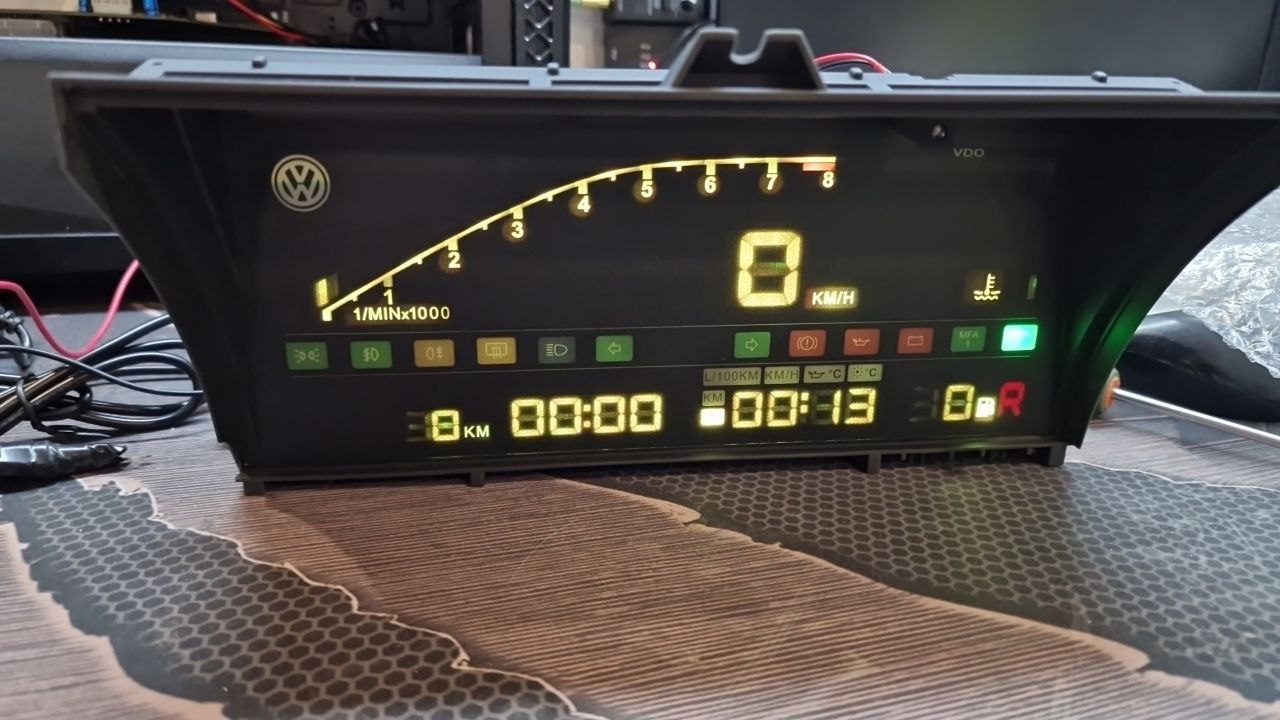
\includegraphics[width=\linewidth]{digifiz_manual/image019.png}
        \caption{Replica Next enclosure and front panel.}
    \end{subfigure}\hfill
    \begin{subfigure}{0.48\textwidth}
        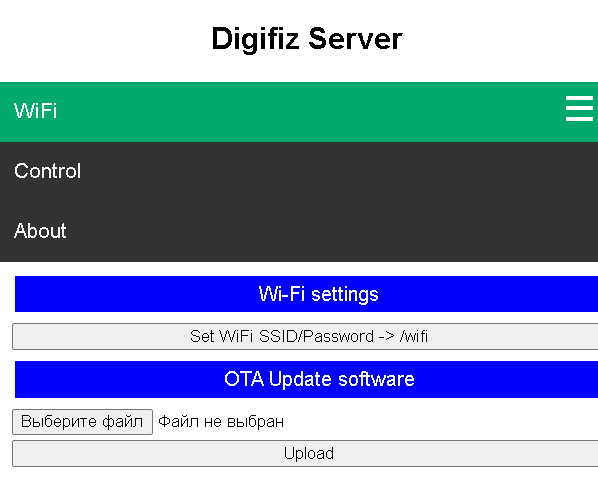
\includegraphics[width=\linewidth]{digifiz_manual/image020.png}
        \caption{Wi-Fi control interface tabs.}
    \end{subfigure}
    \caption{Replica Next hardware and control interface.}
    \label{fig:next-control-tabs}
\end{figure}

\section{Control Tab Overview}

The \emph{Control} tab combines a command entry line, a process button, a result field, quick controls, and buttons to save or reset settings (\Cref{fig:next-control-detail}).
Commands are entered as \verb|<number> <value>| pairs using integer values separated by a space; punctuation and quotation marks are not required.

\begin{figure}[htbp]
    \centering
    \begin{subfigure}{0.48\textwidth}
        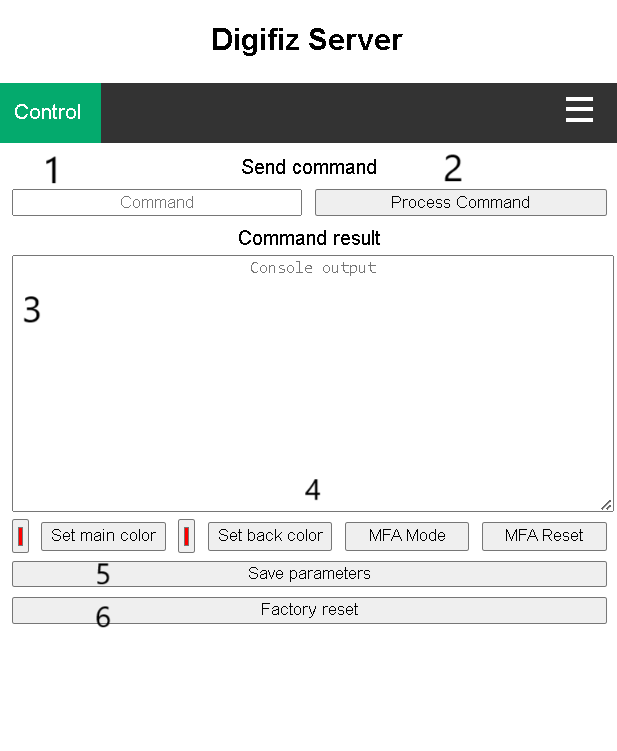
\includegraphics[width=\linewidth]{digifiz_manual/image021.png}
        \caption{Control tab layout with numbered UI elements.}
    \end{subfigure}\hfill
    \begin{subfigure}{0.48\textwidth}
        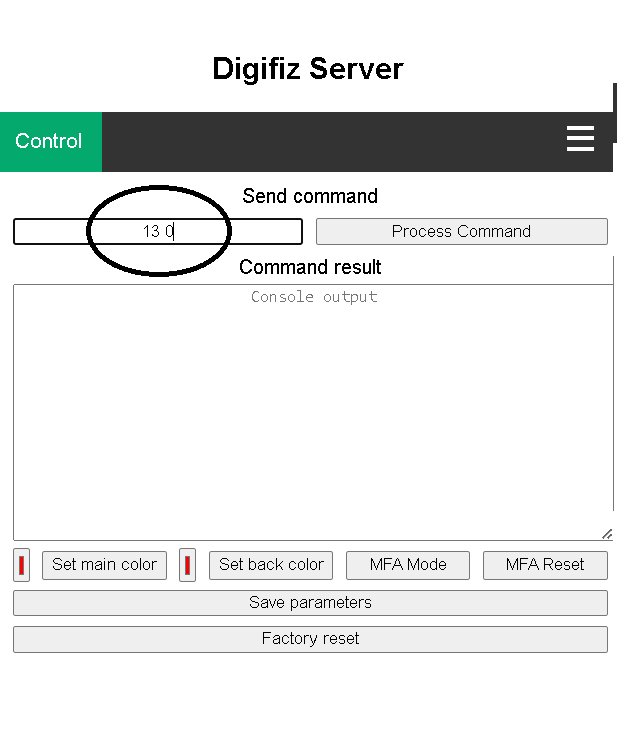
\includegraphics[width=\linewidth]{digifiz_manual/image022.png}
        \caption{Example command entry toggling automatic brightness.}
    \end{subfigure}
    \caption{Replica Next command interface.}
    \label{fig:next-control-detail}
\end{figure}

\section{Command Reference}

\begin{table}[htbp]
    \centering
    \caption{Primary Replica Next configuration commands.}
    \label{tbl:next-commands}
    \begin{tblr}{
        colspec = {>{\ttfamily}Q[c,0.12\linewidth] Q[l] Q[l]},
        row{1} = {font=\bfseries},
        rowsep = 2pt,
    }
        \toprule
        Command & Name & Description \\
        \midrule
        22 (or 0) & PARAMETER\_RPMCOEFFICIENT & Engine RPM calibration factor (100--10000). \\
        1  & PARAMETER\_SPEEDCOEFFICIENT & Speed calibration factor (10--255). \\
        2  & PARAMETER\_COOLANTTHERMISTORB & Coolant thermistor beta coefficient (2000--5000). \\
        3  & PARAMETER\_OILTHERMISTORB & Oil thermistor beta coefficient (2000--5000). \\
        4  & PARAMETER\_AIRTHERMISTORB & Ambient thermistor beta coefficient (2000--5000). \\
        5  & PARAMETER\_TANKMINRESISTANCE & Minimum fuel sender resistance (0--1000~\ohm). \\
        6  & PARAMETER\_TANKMAXRESISTANCE & Maximum fuel sender resistance (100--1000~\ohm). \\
        7  & PARAMETER\_TAU\_COOLANT & Coolant temperature filter constant (1--50, higher is more responsive). \\
        8  & PARAMETER\_TAU\_OIL & Oil temperature filter constant (1--50). \\
        9  & PARAMETER\_TAU\_AIR & Ambient temperature filter constant (1--50). \\
        10 & PARAMETER\_TAU\_TANK & Fuel level filter constant (1--50). \\
        11 & PARAMETER\_MILEAGE & Total odometer value (0--999999). \\
        12 & PARAMETER\_DAILY\_MILEAGE & Trip odometer (0--9999). \\
        13 & PARAMETER\_AUTO\_BRIGHTNESS & Automatic brightness enable (1=on, 0=off). \\
        14 & PARAMETER\_BRIGHTNESS\_LEVEL & Manual brightness level (0--60\%; avoid values above 60). \\
        15 & PARAMETER\_TANK\_CAPACITY & Fuel tank capacity in litres (0--99; 55~L typical for Golf~2). \\
        16 & PARAMETER\_MFA\_STATE & Active MFA mode (normally controlled via hardware input). \\
        17 & PARAMETER\_BUZZER\_OFF & Disable buzzer (1 disables, 0 enables; buzzer absent on Replica Next). \\
        18 & PARAMETER\_MAX\_RPM & Tachometer scaling (typical 8000, range 4000--16000). \\
        19 & PARAMETER\_NORMAL\_RESISTANCE\_COOLANT & Coolant sensor resistance at 25\,^{\circ}C (1000--10000~\ohm). \\
        20 & PARAMETER\_NORMAL\_RESISTANCE\_OIL & Oil sensor resistance at 25\,^{\circ}C (1000--10000~\ohm). \\
        21 & PARAMETER\_NORMAL\_RESISTANCE\_AMB & Ambient sensor resistance at 25\,^{\circ}C (1000--10000~\ohm). \\
        23 & PARAMETER\_DOT\_OFF & Clock colon behaviour (0=blink, 1=solid). \\
        24 & PARAMETER\_BACKLIGHT\_ON & Enable backlight on low beam (not used on Replica Next). \\
        25 & PARAMETER\_M\_D\_FILTER & Median filter parameter (not used on Replica Next). \\
        26 & PARAMETER\_COOLANT\_MAX\_R & Coolant sensor threshold for full-scale indication (100--150\,^{\circ}C). \\
        27 & PARAMETER\_COOLANT\_MIN\_R & Coolant sensor threshold for ``1~bar'' indication (0--80\,^{\circ}C). \\
        31 & PARAMETER\_MAINCOLOR\_R & Red component of UI colour (0--255). \\
        32 & PARAMETER\_MAINCOLOR\_G & Green component of UI colour (0--255). \\
        33 & PARAMETER\_MAINCOLOR\_B & Blue component of UI colour (0--255). \\
        37 & PARAMETER\_RPM\_FILTER & RPM filter aggressiveness (10--200, higher reacts faster). \\
        128 & PARAMETER\_READ\_ADDITION & Read modifier; add 128 to a command to query its current value. \\
        255 & PARAMETER\_SET\_HOUR & Set clock hours (24-hour format). \\
        254 & PARAMETER\_SET\_MINUTE & Set clock minutes. \\
        253 & PARAMETER\_RESET\_DAILY\_MILEAGE & Reset trip odometer. \\
        252 & PARAMETER\_RESET\_DIGITAL & Factory reset of stored parameters. \\
        \bottomrule
    \end{tblr}
\end{table}

\section{Default Parameter Values}

\begin{table}[htbp]
    \centering
    \caption{Replica Next default settings.}
    \label{tbl:next-defaults}
    \begin{tblr}{
        colspec = {>{\ttfamily}Q[c,0.18\linewidth] Q[c,0.18\linewidth] Q[l]},
        row{1} = {font=\bfseries},
        rowsep = 2pt,
    }
        \toprule
        Parameter & Default & Notes \\
        \midrule
        PARAMETER\_RPMCOEFFICIENT & 3000 & RPM coefficient (Audi clusters use 3000). \\
        PARAMETER\_SPEEDCOEFFICIENT & 100 & Calibrated for 100~km/h. \\
        PARAMETER\_COOLANTTHERMISTORB & 4000 &  \\
        PARAMETER\_OILTHERMISTORB & 4000 &  \\
        PARAMETER\_AIRTHERMISTORB & 3812 & 3600 for Gen~2 panels. \\
        PARAMETER\_TANKMINRESISTANCE & 35 & Ohms. \\
        PARAMETER\_TANKMAXRESISTANCE & 265 & Ohms. \\
        PARAMETER\_TAU\_COOLANT & 2 & Filter constant. \\
        PARAMETER\_TAU\_OIL & 2 & Filter constant. \\
        PARAMETER\_TAU\_AIR & 2 & Filter constant. \\
        PARAMETER\_TAU\_TANK & 2 & Filter constant. \\
        PARAMETER\_MILEAGE & Vehicle-specific & Retains stored odometer. \\
        PARAMETER\_DAILY\_MILEAGE & 0 &  \\
        PARAMETER\_AUTO\_BRIGHTNESS & 1 & Enabled. \\
        PARAMETER\_BRIGHTNESS\_LEVEL & 25 & Gen~2 typical value; Gen~1/1.5 use 7 or 13. \\
        PARAMETER\_TANK\_CAPACITY & 63 & Litres. \\
        PARAMETER\_MFA\_STATE & 0 & Default MFA page. \\
        PARAMETER\_BUZZER\_OFF & 1 & Buzzer disabled. \\
        PARAMETER\_MAX\_RPM & 8000 & Tachometer scale. \\
        PARAMETER\_NORMAL\_RESISTANCE\_COOLANT & 1000 & Ohms at 25\,^{\circ}C. \\
        PARAMETER\_NORMAL\_RESISTANCE\_OIL & 1000 & Ohms at 25\,^{\circ}C. \\
        PARAMETER\_NORMAL\_RESISTANCE\_AMB & 2991 & 500~\ohm{} for Gen~2 sensors. \\
        PARAMETER\_DOT\_OFF & 0 & Blinking clock colon. \\
        PARAMETER\_BACKLIGHT\_ON & 1 & Backlight enabled with low beam. \\
        PARAMETER\_M\_D\_FILTER & 65535 & Legacy median filter constant. \\
        PARAMETER\_COOLANT\_MAX\_R & 120 & \(^{\circ}\mathrm{C}\). \\
        PARAMETER\_COOLANT\_MIN\_R & 60 & \(^{\circ}\mathrm{C}\). \\
        PARAMETER\_MAINCOLOR\_R & 180 & Yellow-green default. \\
        PARAMETER\_MAINCOLOR\_G & 240 & Yellow-green default. \\
        PARAMETER\_MAINCOLOR\_B & 6 & Yellow-green default. \\
        PARAMETER\_RPM\_FILTER & 70 & Filter speed. \\
        PARAMETER\_UPTIME & 0 & Runtime counter. \\
        \bottomrule
    \end{tblr}
\end{table}

\section{Reading Parameters and Examples}

To read a parameter, add 128 to the command number (for example, \verb|129 0| reads the current speed coefficient).
Typical configuration commands include disabling automatic brightness (\verb|13 0|), re-enabling it (\verb|13 1|), adjusting speed calibration (\verb|1 110| increases displayed speed by 5\%), and setting the odometer (\verb|11 123456|).
Clock values are set with \verb|255 <hours>| and \verb|254 <minutes>|.
Colour adjustments use commands 31--33 to set the RGB channels.

\section{Service Commands}

Recent firmware revisions accept human-readable parameter names (for example, \verb|PARAMETER_RPMCOEFFICIENT 3000|).
The diagnostic command \verb|adc 0| prints raw ADC readings for sensor troubleshooting.
Colour configuration can also be performed using the visual controls added in the latest releases; update the firmware through the \emph{WiFi} tab to access these features.
